%%%%%%%%%%%%%%%%%%%%%%%%%
%% Header for standard beamer presentation
%%
%%  PresentationHeader.tex
%%
%%%%%%%%%%%%%%%%%%%%%%%%%

\documentclass[english,10pt]{beamer}

%%%%%%%%%%%%%%%%%%%%
%% Include general header where common packages are defined
%%%%%%%%%%%%%%%%%%%%

% general packages without options
\usepackage{amsmath,amssymb,bbm}




%%%%%%%%%%%%%%%%%%%%
%% Idem general commands
%%%%%%%%%%%%%%%%%%%%

%%% Commands

\newcommand{\noun}[1]{\textsc{#1}}


%% Math

% Operators
\DeclareMathOperator{\Cov}{Cov}
\DeclareMathOperator{\Var}{Var}
\DeclareMathOperator{\E}{\mathbb{E}}
\DeclareMathOperator{\Proba}{\mathbb{P}}

\newcommand{\Covb}[2]{\ensuremath{\Cov\!\left[#1,#2\right]}}
\newcommand{\Eb}[1]{\ensuremath{\E\!\left[#1\right]}}
\newcommand{\Pb}[1]{\ensuremath{\Proba\!\left[#1\right]}}
\newcommand{\Varb}[1]{\ensuremath{\Var\!\left[#1\right]}}

% norm
\newcommand{\norm}[1]{\| #1 \|}


% amsthm environments
\newtheorem{definition}{Definition}



%% graphics

% renew graphics command for relative path providment only ?
%\renewcommand{\includegraphics[]{}}






\usetheme{Warsaw}

\setbeamertemplate{footline}[text line]{}
\setbeamercolor{structure}{fg=purple!50!blue, bg=purple!50!blue}

\setbeamercovered{transparent}


% shortened command for a justified frame
\newcommand{\jframe}[2]{\frame{\frametitle{#1}\justify{#2}}}



%%%%%%%%%%%%%%%%%%%%%
%% Begin doc
%%%%%%%%%%%%%%%%%%%%%

\begin{document}



\title{Thesis Progress Meeting}


\author{J.~Raimbault$^{1,2}$}

\institute{$^{1}$G{\'e}ographie-cit{\'e}s (UMR 8504 CNRS)\\
$^{2}$LVMT (UMR-T 9403 IFSTTAR)}


\date{January 26th 2016}


%%%%%%%%%%%%%%%%%%%%%%%%%%%%%%%%
\begin{frame}
\titlepage
\end{frame}

%\begin{frame}
%\tableofcontents
%\end{frame}
%%%%%%%%%%%%%%%%%%%%%%%%%%%%%%%%


%\section{Projects Organization}

%\jframe{Projects Organization}{
%   \includegraphics[width=\textwidth,height=0.8\textheight]{figures/orgaProjects}
%}



\section{Achieved Work}


\jframe{Achieved Work (by projects)}{
\begin{itemize}
\item Biblio/Meetings/Organisation [0.7w]
\item Conference [0.7w]
\item Reading Records (\emph{Synergetics}) [0.2w]
\item Monitorat [1,3w]
\item Cybergeo Project [1w]
\item Correlated Synthetic data [3w]
\item Theory construction [0.2w]
\item BP Case Study / Spatial Econometrics [0,3w]
\end{itemize}

}



\section{Correlated Synthetic Data}

\sframe{Context}{
\textbf{Def. : } \emph{Synthetic Data} are output of generative models (and possibly inputs of models using them).
\medskip

Methodology used in various fields, e.g. therapeutic evaluation~\cite{abadie2010synthetic}, territorial systems analysis~\cite{moeckel2003creating,pritchard2009advances}, machine learning~\cite{bolon2013review} or bio-informatics~\cite{van2006syntren}.

\medskip

Few examples at the second order : specific examples as~\cite{ye2011investigation} for discrete choices ; methods that can be interpreted this way : generation of complex networks~\cite{newman2003structure}.

}



%%%%%%%%%%%%%%%%%
\sframe{Generic Method}{
$\vec{X}_I$ multidimensional stochastic process, $\mathbf{X}=(X_{i,j})$ realizations. 

\bigskip

\textbf{Aim : } Generate a statistical population $\mathbf{\tilde{X}}=\tilde{X}_{i,j}$ such that:
\medskip
\begin{enumerate}
\item proximity to data : given a precision $\varepsilon$ and an indicator $f$, $\norm{f(\mathbf{X})-f(\mathbf{\tilde{X}})} < \varepsilon$
\item control of the estimated correlation structure : $\hat{\Var{}}\left[(\tilde{X}_i)\right] = \Sigma R$ with $R$ fixed.
\end{enumerate}

}


%%%%%%%%%%%%%%%%%
\sframe{Geographical data : Context and Objective}{

\begin{itemize}
\jitem{In geography, generation of synthetic populations for agent-based models~\cite{pritchard2009advances}.}
\jitem{Generation of spatial synthetic configuration not used (Geo. Weighted Regression~\cite{brunsdon1998geographically} can be interpreted this way) ; however crucial for abstract models~\cite{schmitt2014modelisation}}
\jitem{\cite{cottineau2015revisiting} recently proposed to estimate the sensitivity of spatial models of simulation to initial configuration (application to Schelling model).}
\jitem{Case study : city-transportation interactions, complex to understood quantitatively~\cite{offner1993effets,bretagnolle:tel-00459720} $\rightarrow$ simple model of population density and transportation network morphogenesis.}
\end{itemize}
}



%%%%%%%%%%%%%%%%%
\sframe{Modèle}{
\footnotesize
Simple coupling between
\begin{itemize}
\jitem{Iterative generation of a density grid by preferential attachment/diffusion~\cite{raimbault2016calibration},  calibrated on morphological objectives on european density grid.}
\jitem{Heuristic network generation conditional to density :
\begin{itemize}
\footnotesize
\item Distribution of a fixed number of centers preferentially following density
\item Deterministic percolation between closest neighbors
\item Breaking of interaction potentials
\[
V_{ij}(d) = \left[ (1 - k_h) + k_h \cdot \left( \frac{P_i P_j}{P^2} \right)^{\gamma} \right]\cdot \exp{\left( -\frac{d}{r_g (1 + d/d_0)} \right)}
\]
for a fixed number of couples $N_L$ such that $V_{ij}(d_N)/V_{ij}(d_{ij})$ is minimal among $K\cdot N_L$ strongest euclidian potentials ($K=5$ fixed)
\item Planarization
\end{itemize}
}
\end{itemize}
Indicators : morphology~\cite{le2015forme} (Moran, mean distance, entropy, hierarchy) and network (centrality, mean width, speed, diameter).

}

%%%%%%%%%%%%%%%%%
\sframe{Implementation and Exploration}{

$\rightarrow$ Formal and Operational coupling : modular implementation (\texttt{scala}/\texttt{NetLogo}) encapsulated by \texttt{OpenMole}~\cite{reuillon2013openmole}

\bigskip

$\rightarrow$ Exploration by intensive computation on grid via \texttt{OpenMole} : calibration of density model alone ($\sim 1.5\cdot 10^6$ runs) ; brutal exploration by LHS sampling for feasible correlations ($\sim 5\cdot 10^4$ runs) 

}



%%%%%%%%%%%%%%%%%
\sframe{Results : Density Model alone}{
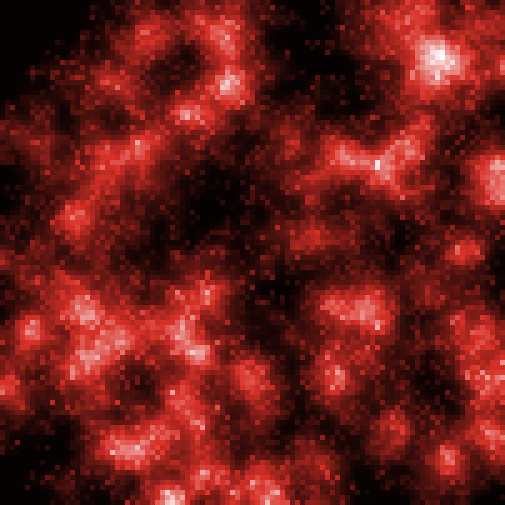
\includegraphics[width=0.24\textwidth]{figures/density/conf1}\hspace{0.1em}
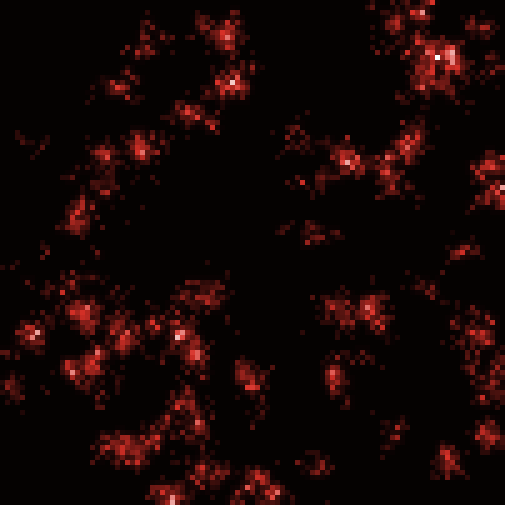
\includegraphics[width=0.24\textwidth]{figures/density/conf2}\hspace{0.1em}
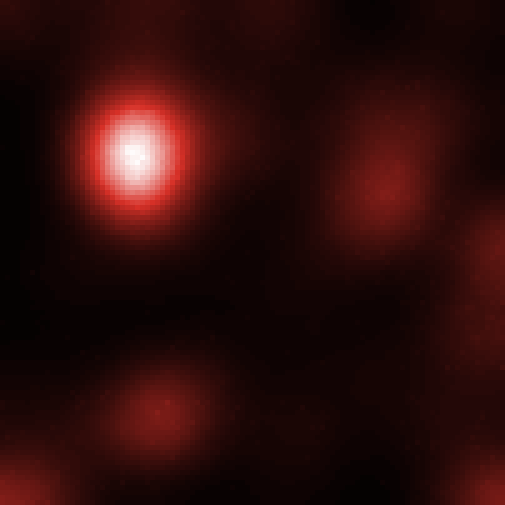
\includegraphics[width=0.24\textwidth]{figures/density/conf3}\hspace{0.1em}
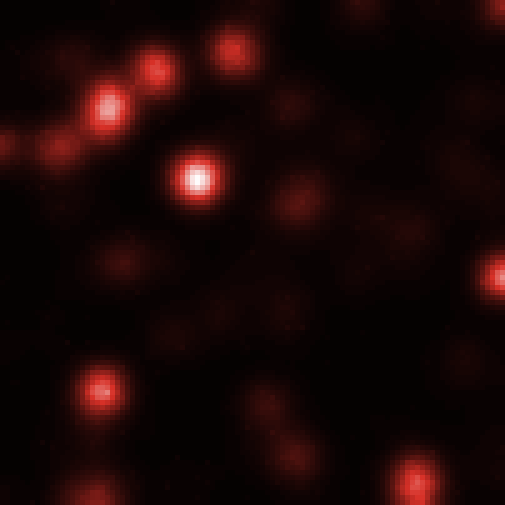
\includegraphics[width=0.24\textwidth]{figures/density/conf4}\hspace{0.1em}
\\
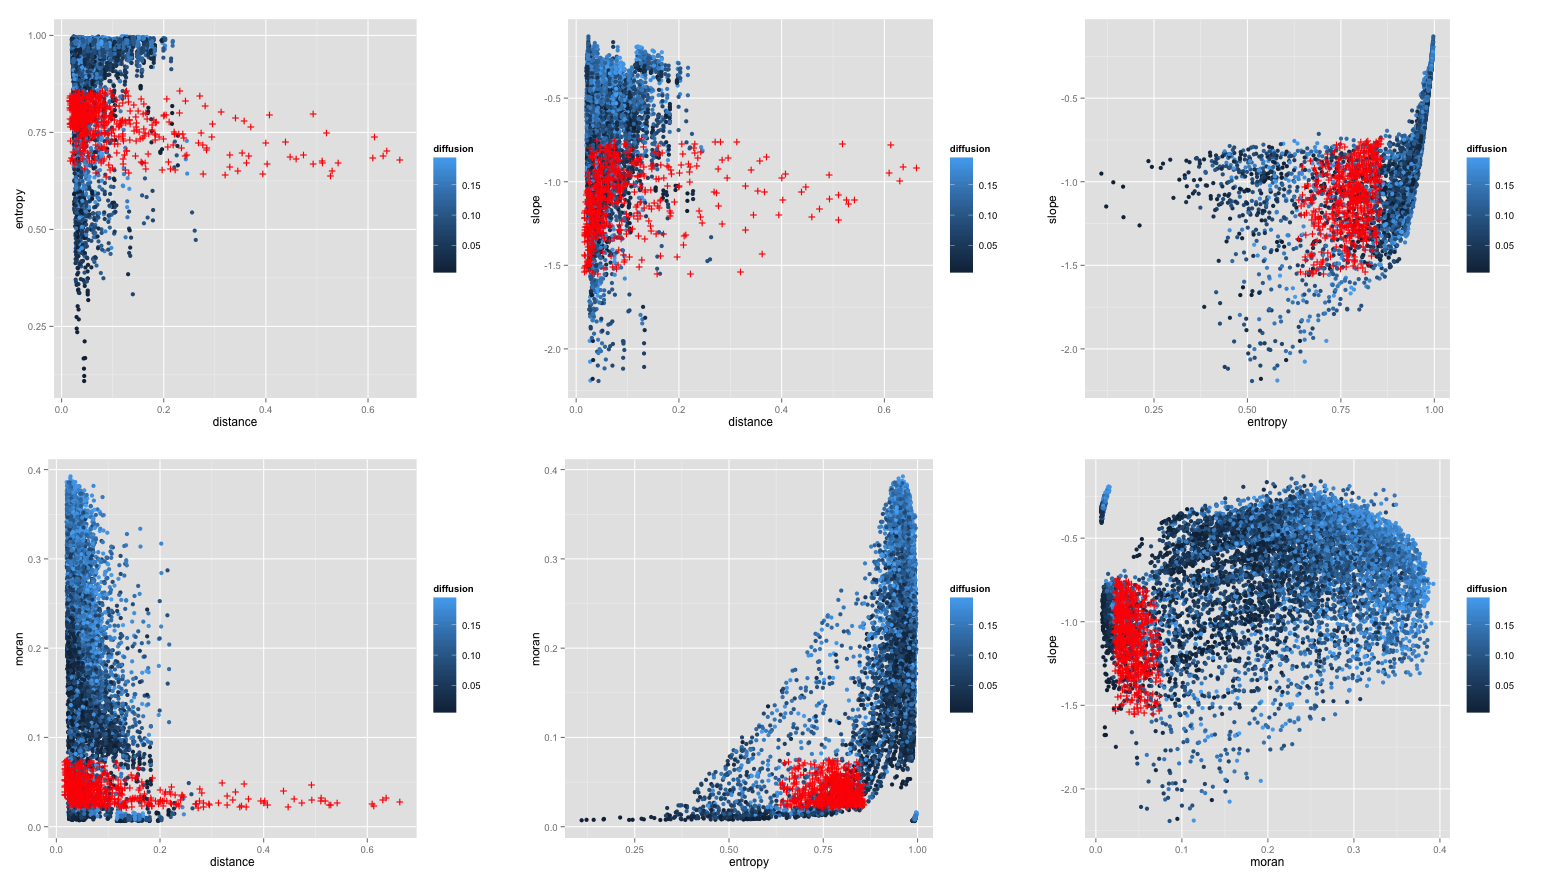
\includegraphics[width=0.5\textwidth,height=0.55\textheight]{figures/density/scatt}
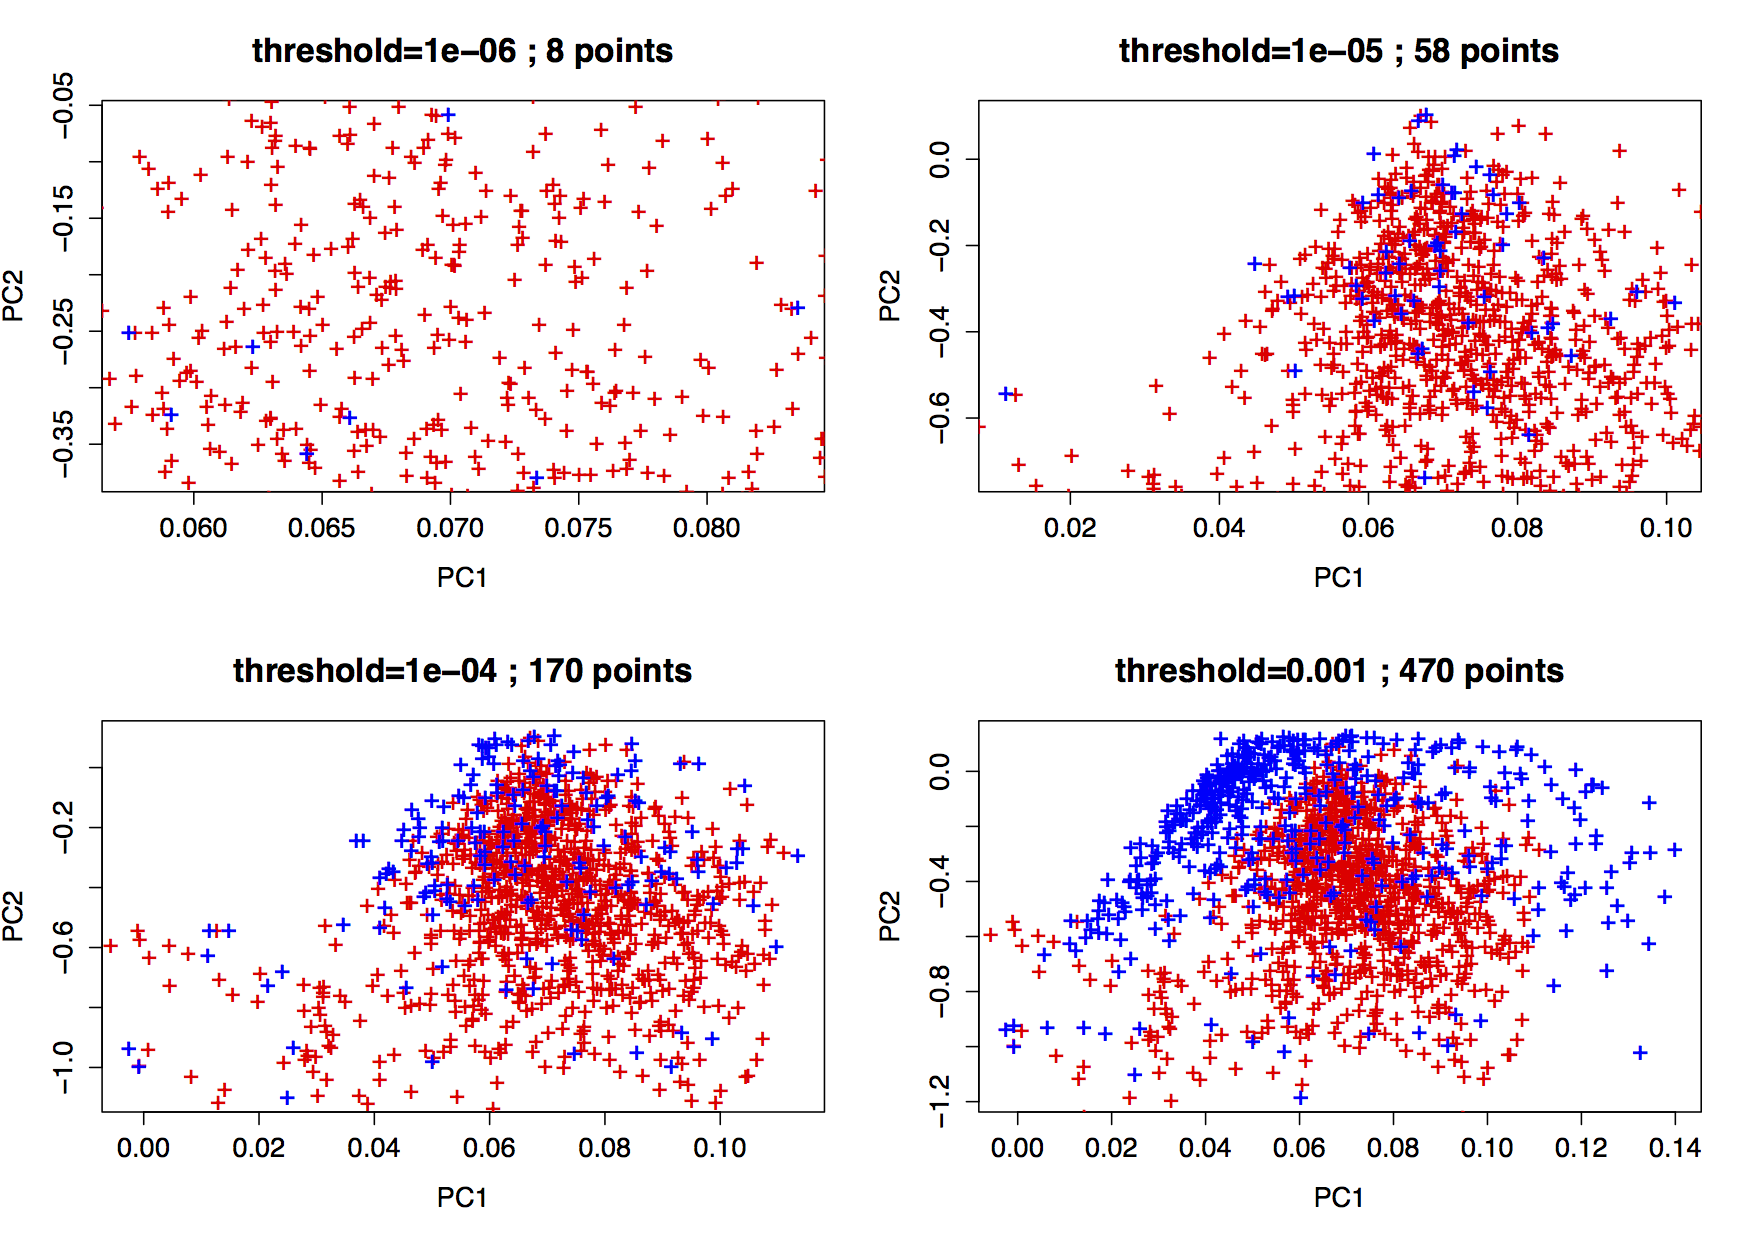
\includegraphics[width=0.5\textwidth,height=0.55\textheight]{figures/density/pca}
}



%%%%%%%%%%%%%%%%%
\sframe{Results : examples of configurations}{
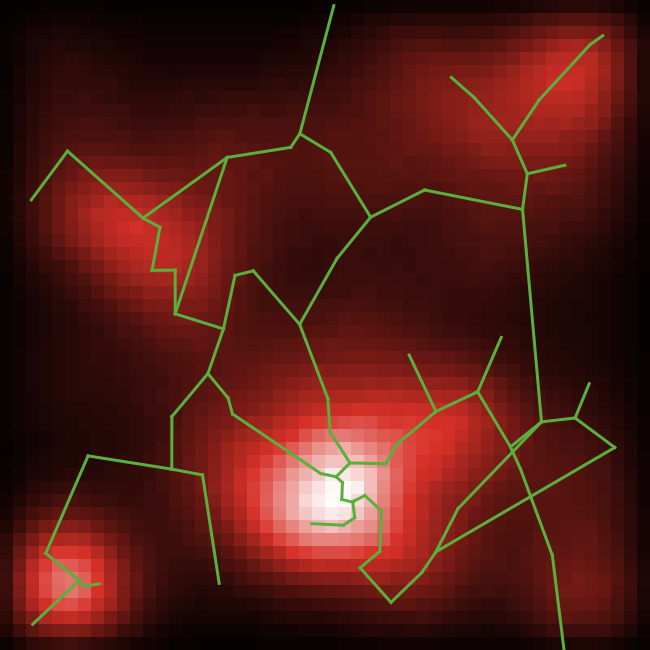
\includegraphics[width=0.49\textwidth]{figures/configs/2_param71913_seed10}\hspace{0.1cm}
   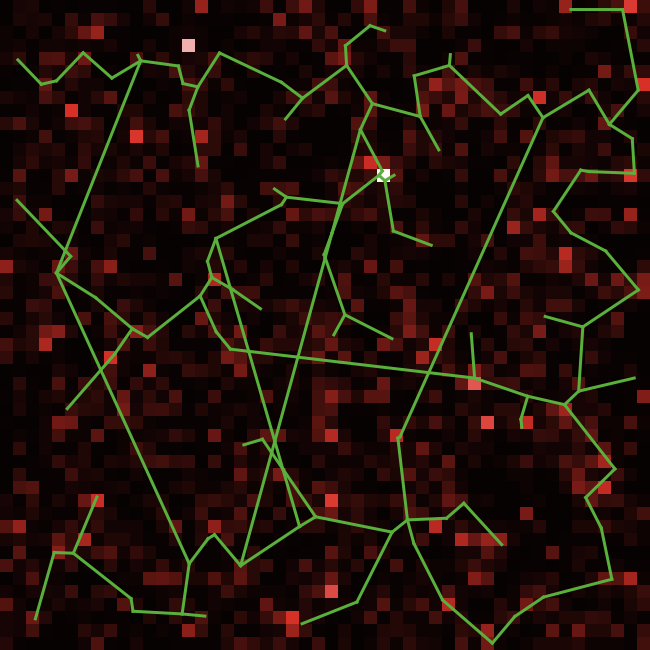
\includegraphics[width=0.49\textwidth]{figures/configs/3_param71918_seed0}
}

%%%%%%%%%%%%%%%%%
\sframe{Results : examples of configurations}{
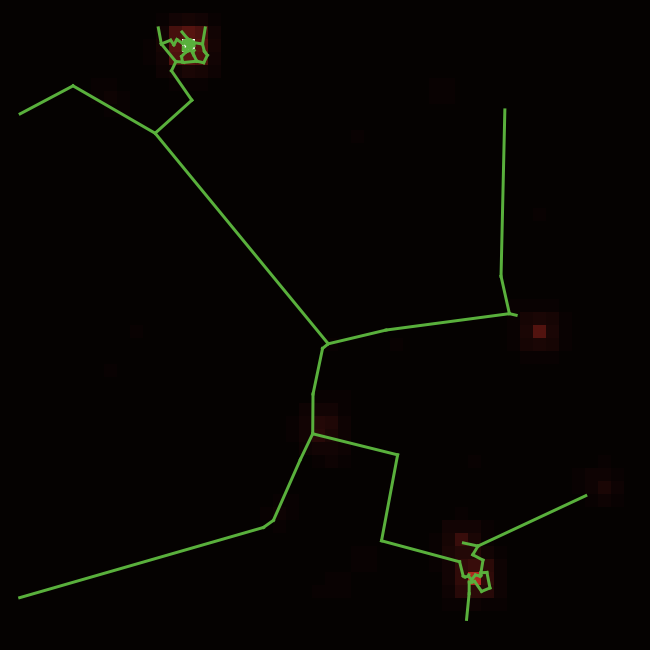
\includegraphics[width=0.49\textwidth]{figures/configs/1_param71861_seed0}\hspace{0.1cm}
   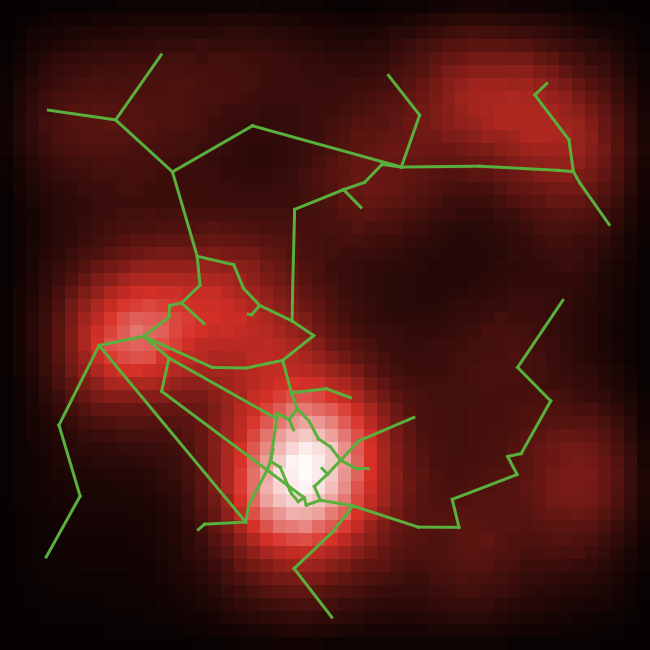
\includegraphics[width=0.49\textwidth]{figures/configs/4_param71945_seed0}
}




%%%%%%%%%%%%%%%%%
\sframe{Results : cross-correlations}{
\centering
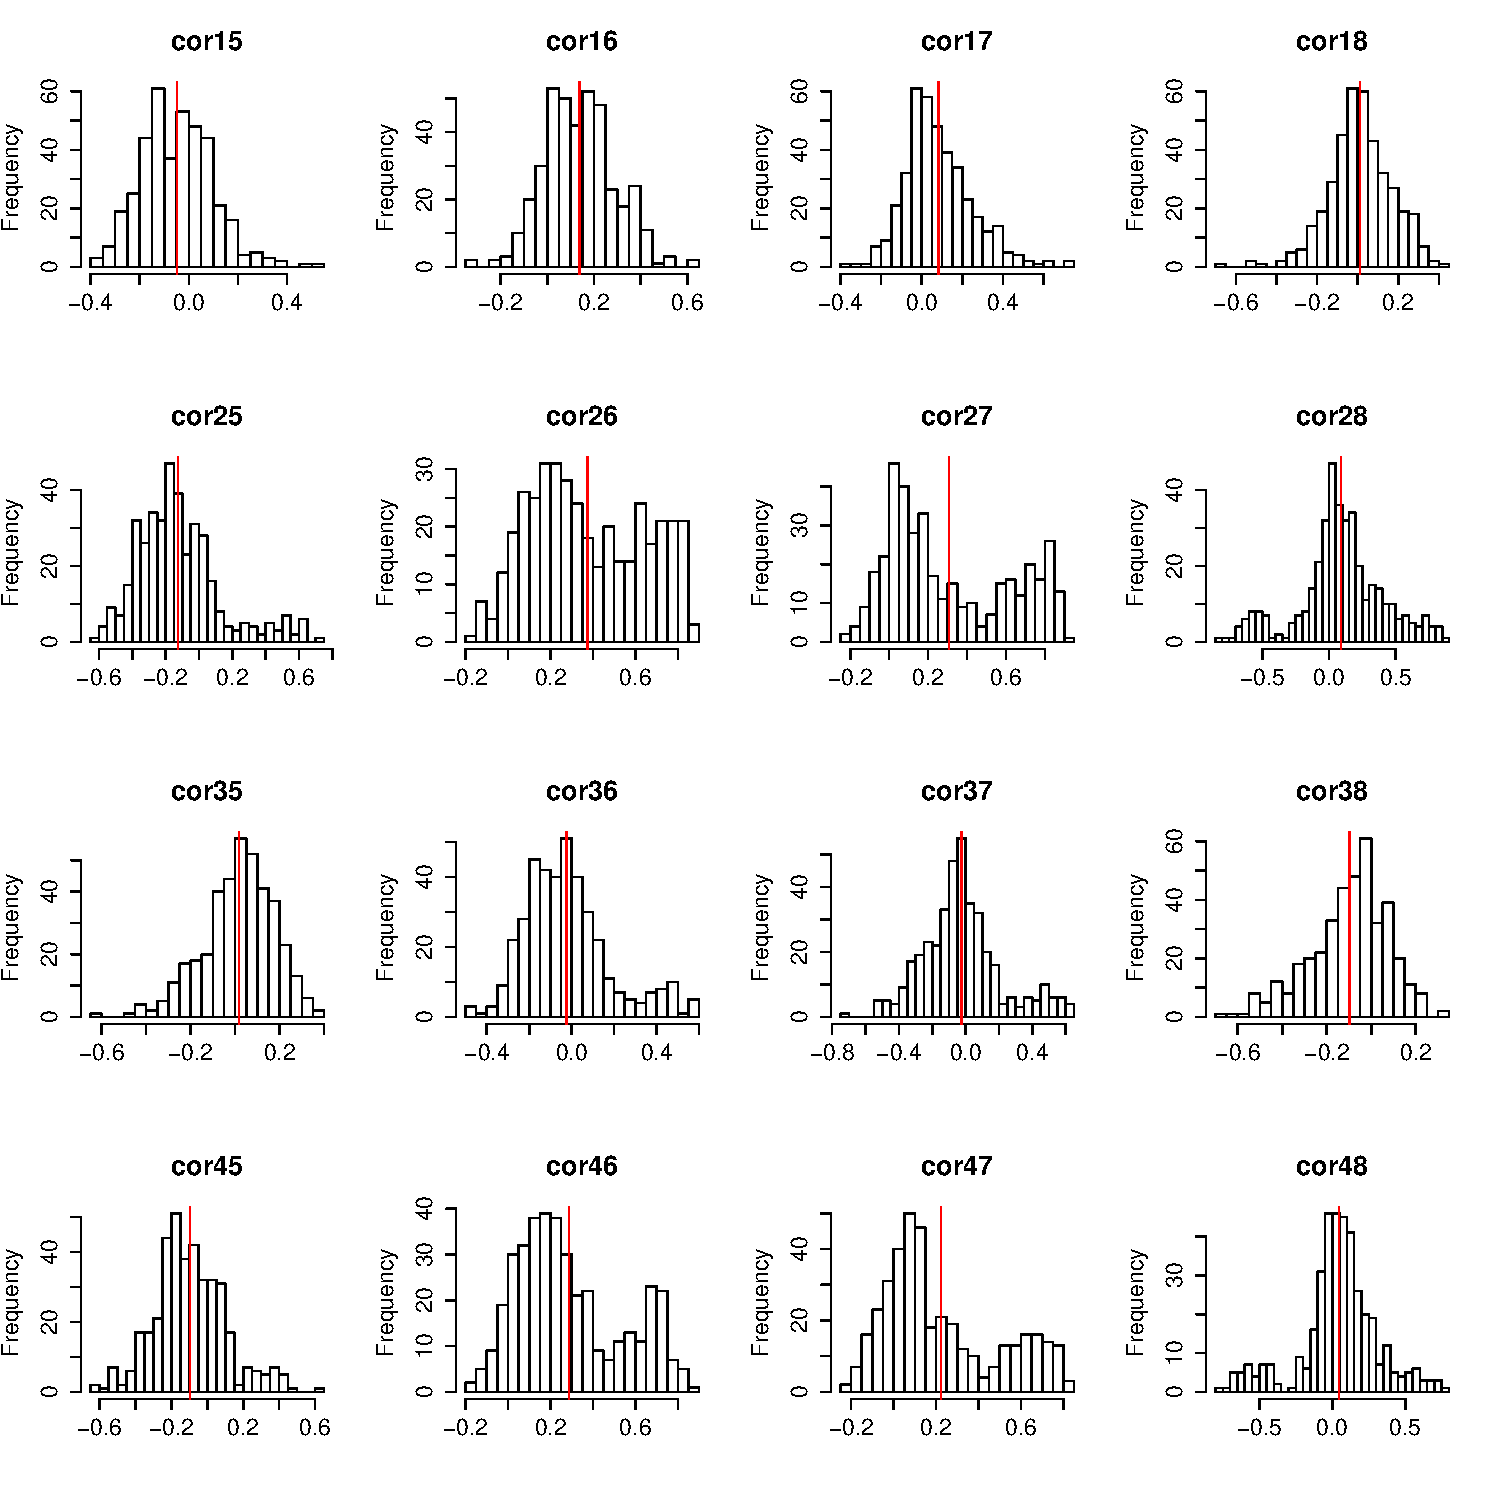
\includegraphics[height=0.85\textheight]{figures/hist_crossCorMat_breaks30}
}

%%%%%%%%%%%%%%%%%
\sframe{Results : feasible correlations}{
\textit{Mean matrices in a principal plan}

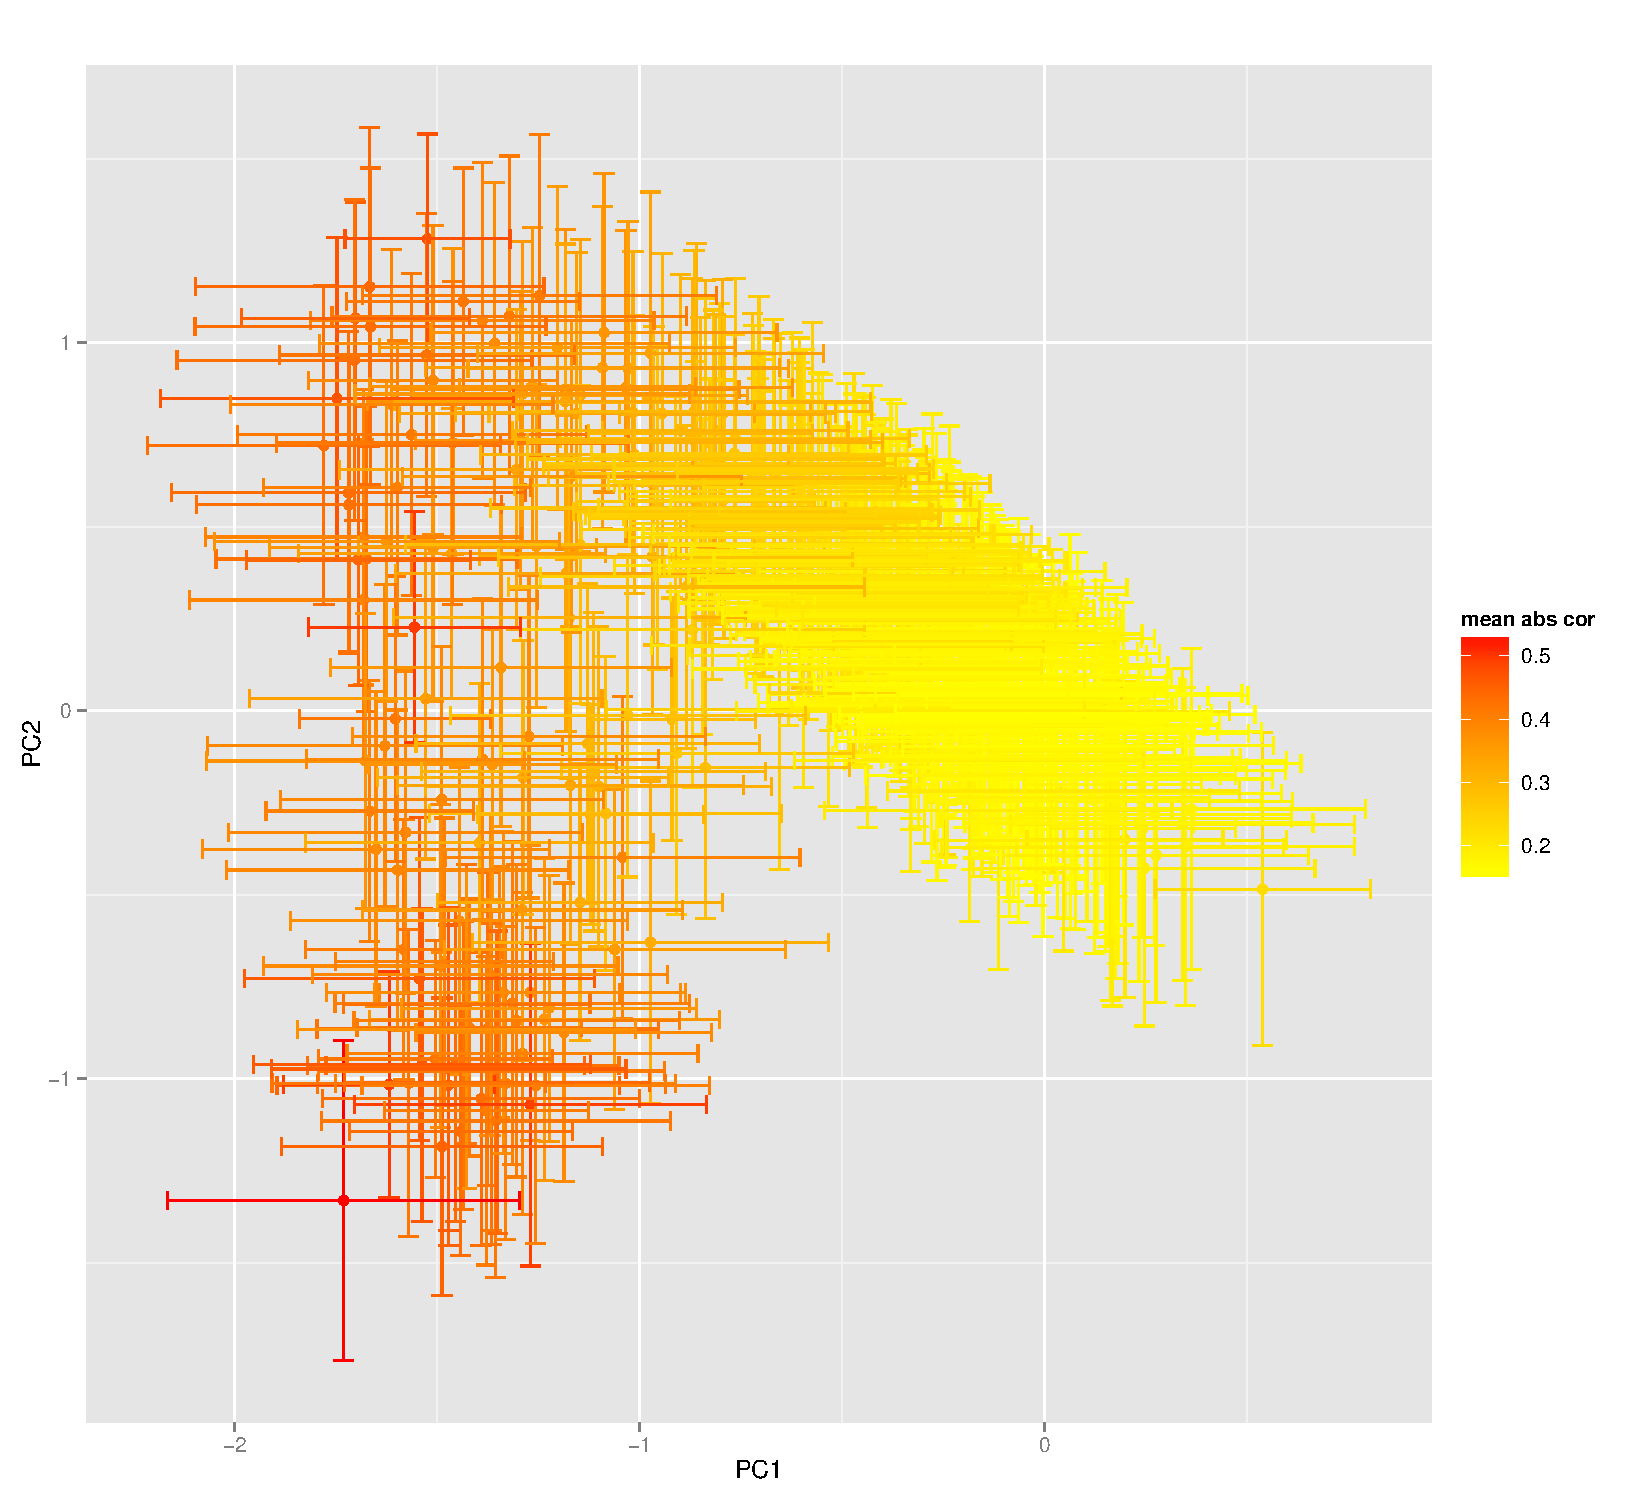
\includegraphics[width=0.5\textwidth,height=0.65\textheight]{figures/pca_meanAbsCor_errorBars}
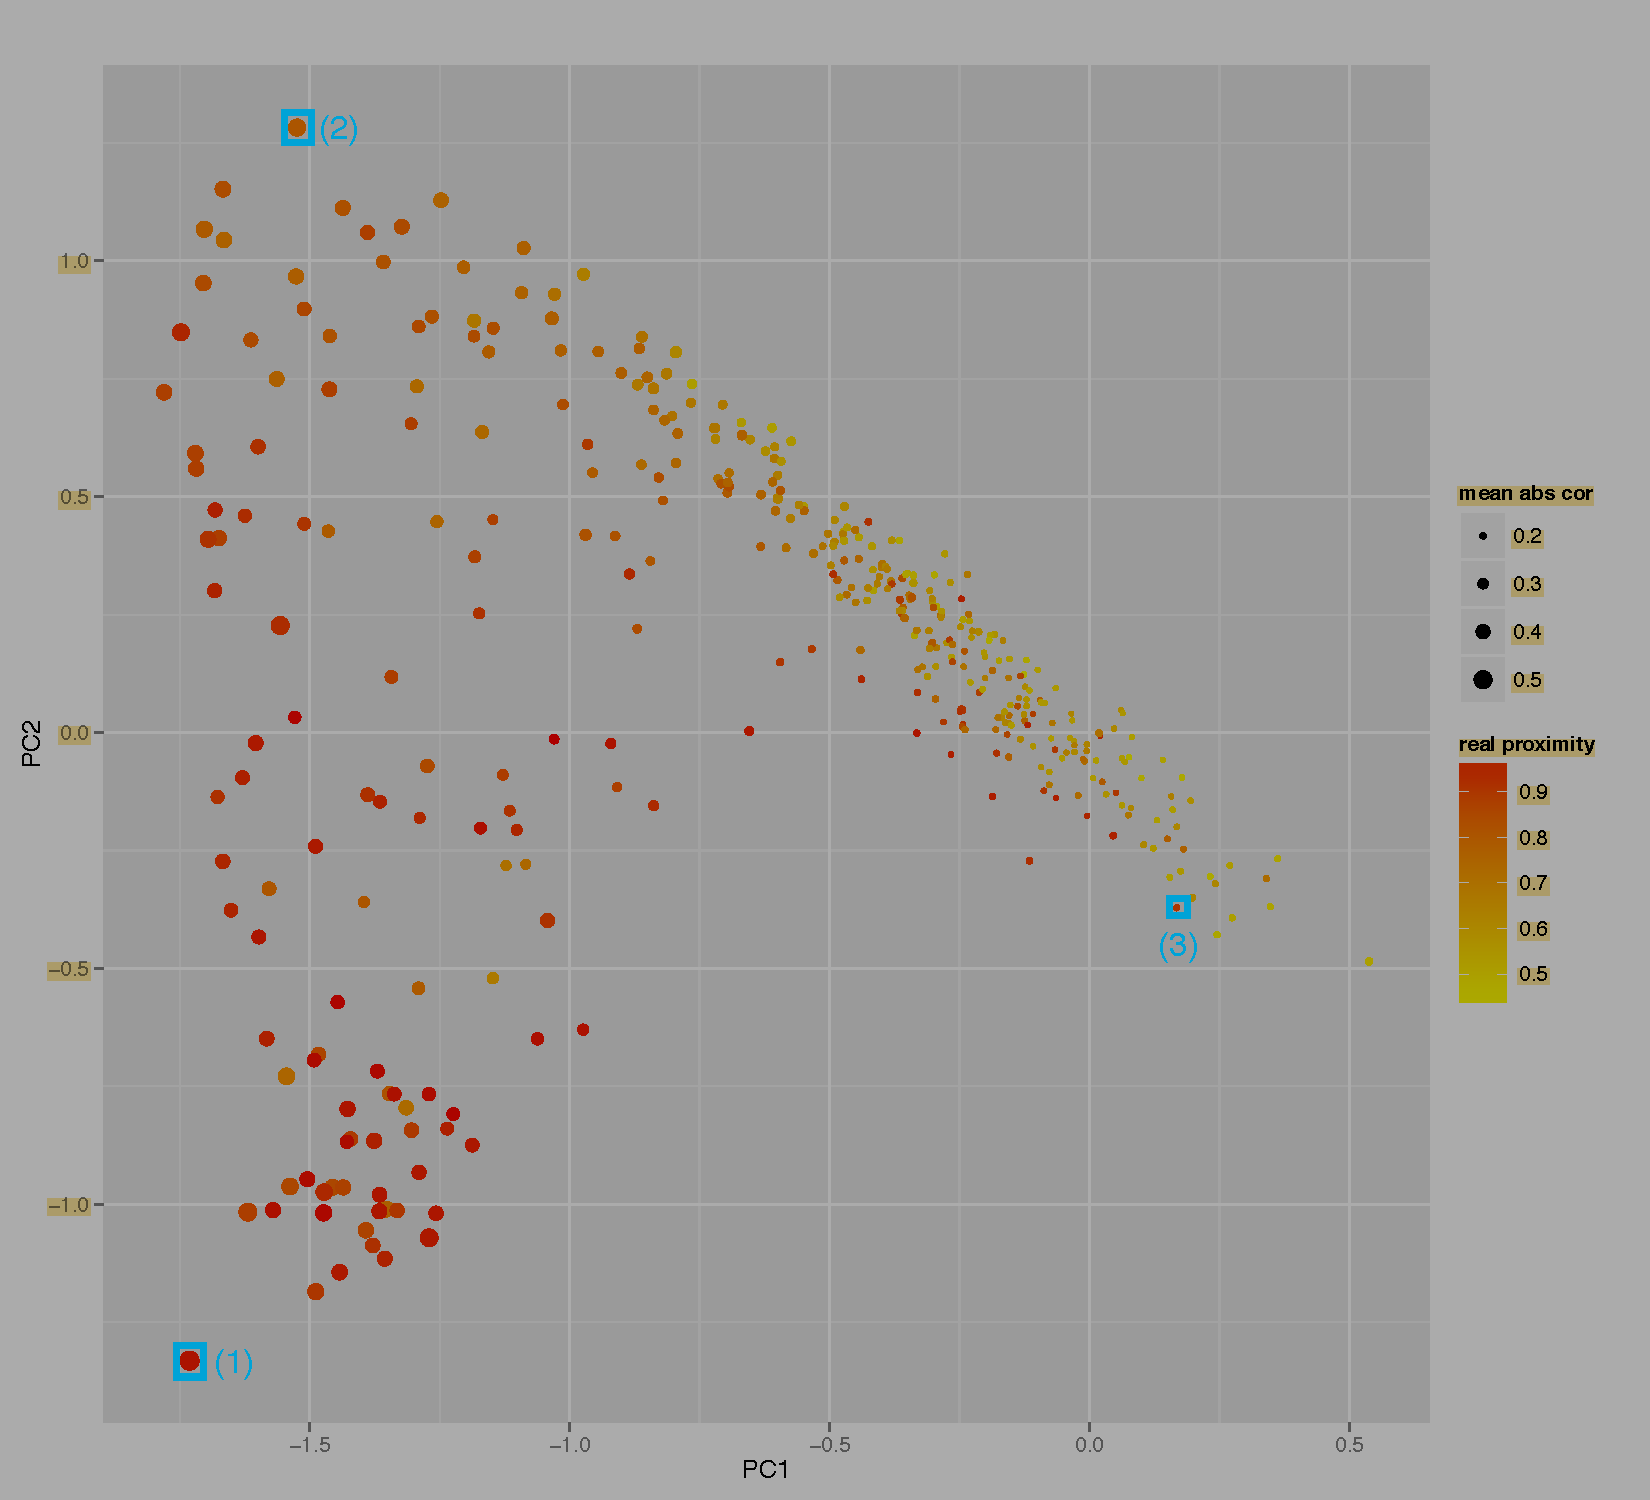
\includegraphics[width=0.5\textwidth,height=0.65\textheight]{figures/pca_realDistCol_meanAbsCorSize_withSpecificPoints}
}

%%%%%%%%%%%%%%%%%
\sframe{Results : exemples of correlations}{
\begin{columns}[T] % align columns
\begin{column}{.48\textwidth}
\centering
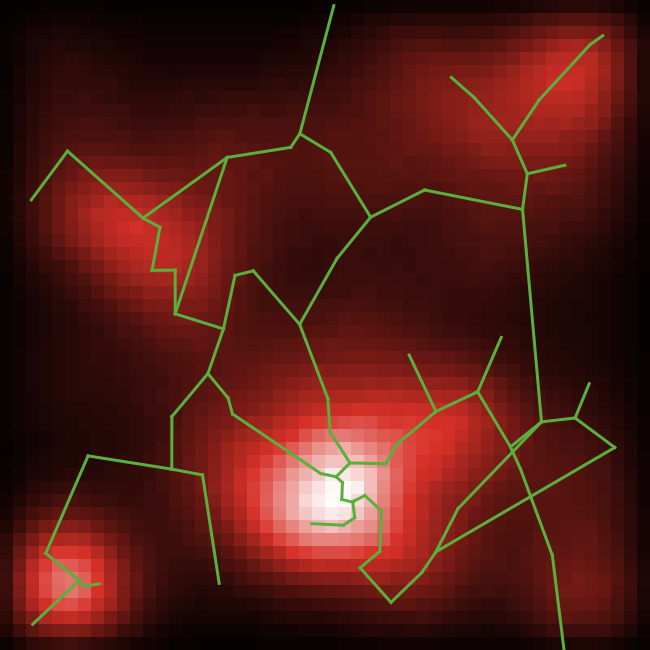
\includegraphics[width=\textwidth]{figures/configs/2_param71913_seed10}\\
$\rho[\bar{d},\bar{c}]\simeq 0.34$
\end{column}%
\hfill%
\begin{column}{.48\textwidth}
\centering
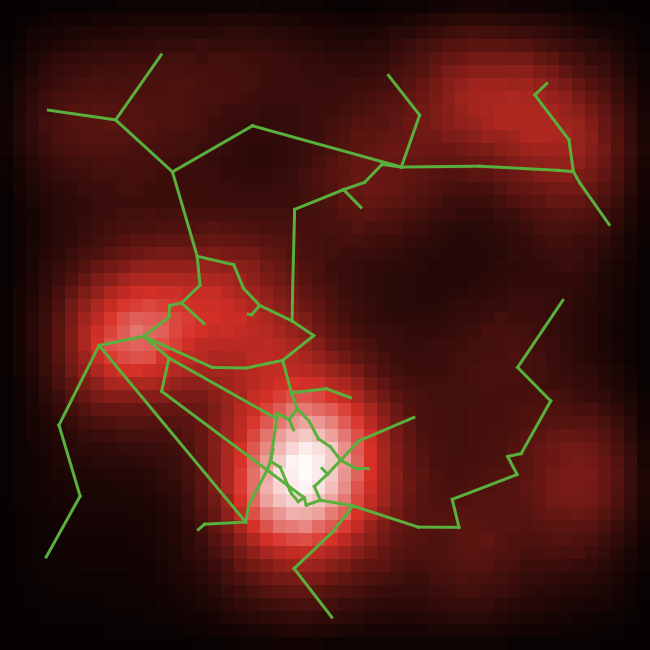
\includegraphics[width=\textwidth]{figures/configs/4_param71945_seed0}\\
$\rho[\bar{d},\bar{c}]\simeq-0.41$
\end{column}%
\end{columns}

$\rightarrow$ \textit{gravity hierarchy more important in (1) $\gamma=3.9,k_h=0.7$ against $\gamma=1.07,k_h=0.25$ for (2)}

}



%%%%%%%%%%%%%%%%%
\sframe{Applications}{

\begin{enumerate}
\item Calibration of the coupled model, street network data( ¡ edge effects !) $\rightarrow $ generation of correlated synthetic data corresponding to a given urban system $\rightarrow$ intrinsic correlations to be compared to estimated correlations between different states : non-ergodicity of urban systems~\cite{pumain2012urban}).
\item Dynamical correlations in a strongly coupled model / spatio-temporal correlations in a strong spatial coupling.
\end{enumerate}

}


\section{Spatial Econometrics}

\sframe{Context}{

}

\sframe{On Accessibility}{

}

\sframe{Statistical Analysis}{

}





\section{Next Steps}


\sframe{P. Bourgine framework for Complex Adaptive Systems}{

}


%%%%%%%%%%%%%%%%%%%%%%%%%%%%%%%%
\jframe{Next steps (until February 15th 2016)}{
\begin{itemize}
\item Theory exemplification, paper finalization  [1w]\medskip
\item Spatial Econometrics / Case study [0.5w]\medskip
\item Cybergeo [0.5w]\medskip
\item Wrap everything within a 1-year Memoire [1w]\medskip
\end{itemize}
}






%%%%%%%%%%%%%%%%%%%%%%%%%%%%%%%%
\begin{frame}[allowframebreaks]
\frametitle{References}
\bibliographystyle{apalike}
\bibliography{/Users/Juste/Documents/ComplexSystems/CityNetwork/Biblio/Bibtex/CityNetwork,biblio}
\end{frame}
%%%%%%%%%%%%%%%%%%%%%%%%%%%%%%%%


\end{document}